\documentclass[
	ngerman,
	toc=listof, % Abbildungsverzeichnis sowie Tabellenverzeichnis in das Inhaltsverzeichnis aufnehmen
	toc=bibliography, % Literaturverzeichnis in das Inhaltsverzeichnis aufnehmen
	footnotes=multiple, % Trennen von direkt aufeinander folgenden Fußnoten
	parskip=half, % vertikalen Abstand zwischen Absätzen verwenden anstatt horizontale Einrückung von Folgeabsätzen
	numbers=noendperiod % Den letzten Punkt nach einer Nummerierung entfernen (nach DIN 5008)
]{scrartcl}
\pdfminorversion=5 % erlaubt das Einfügen von pdf-Dateien bis Version 1.7, ohne eine Fehlermeldung zu werfen (keine Garantie für fehlerfreies Einbetten!)

\usepackage[utf8]{inputenc} % muss als erstes eingebunden werden, da Meta/Packages ggfs. Sonderzeichen enthalten

\usepackage{listings}
\usepackage{color}
\usepackage{float}

% !TEX root = Index.tex


\newcommand{\titel}{Entwicklung eines Service-Manager}
\newcommand{\untertitel}{Vereinfachte Dienstverwaltung, mithilfe einer intuitiven Oberflächenverwaltung.}
\newcommand{\kompletterTitel}{\titel{} -- \untertitel}

\newcommand{\autorName}{Christopher Rudolf Karl-Heinz Mogler}
\newcommand{\autorAnschrift}{Schramberger Str. 13}
\newcommand{\autorOrt}{77761 Schiltach}

\newcommand{\betriebLogo}{img/logo.png}
\newcommand{\betriebLogoBig}{img/big-logo.png}
\newcommand{\betriebName}{Weiss GmbH Softwarelösungen}
\newcommand{\betriebAnschrift}{Schenkenzeller Str. 163}
\newcommand{\betriebOrt}{77761 Schiltach}

\newcommand{\ausbildungsberuf}{Fachinformatiker für Anwendungsentwicklung}
\newcommand{\betreff}{Dokumentation zur betrieblichen Projektarbeit}
\newcommand{\pruefungstermin}{Sommer 2020}
\newcommand{\abgabeOrt}{Schiltach}
\newcommand{\abgabeTermin}{29.05.2020}
 % Metadaten zu diesem Dokument (Autor usw.)
% !TEX root = ../Index.tex

% Anpassung an Landessprache ---------------------------------------------------
\usepackage{babel}

% Umlaute ----------------------------------------------------------------------
%   Umlaute/Sonderzeichen wie äüöß direkt im Quelltext verwenden (CodePage).
%   Erlaubt automatische Trennung von Worten mit Umlauten.
% ------------------------------------------------------------------------------
\usepackage[T1]{fontenc}
\usepackage{textcomp} % Euro-Zeichen etc.

% Schrift ----------------------------------------------------------------------
\usepackage{lmodern} % bessere Fonts
\usepackage{relsize} % Schriftgröße relativ festlegen

% Tabellen ---------------------------------------------------------------------
\PassOptionsToPackage{table}{xcolor}
\usepackage{tabularx}
% für lange Tabellen
\usepackage{longtable}
\usepackage{array}
\usepackage{ragged2e}
\usepackage{lscape}
\newcolumntype{w}[1]{>{\raggedleft\hspace{0pt}}p{#1}} % Spaltendefinition rechtsbündig mit definierter Breite

% Grafiken ---------------------------------------------------------------------
\usepackage[dvips,final]{graphicx} % Einbinden von JPG-Grafiken ermöglichen
\usepackage{graphics} % keepaspectratio
\usepackage{floatflt} % zum Umfließen von Bildern
\graphicspath{{Bilder/}} % hier liegen die Bilder des Dokuments

% Sonstiges --------------------------------------------------------------------
\usepackage[titles]{tocloft} % Inhaltsverzeichnis DIN 5008 gerecht einrücken
\usepackage{amsmath,amsfonts} % Befehle aus AMSTeX für mathematische Symbole
\usepackage{enumitem} % anpassbare Enumerates/Itemizes
\usepackage{xspace} % sorgt dafür, dass Leerzeichen hinter parameterlosen Makros nicht als Makroendezeichen interpretiert werden

\usepackage{makeidx} % für Index-Ausgabe mit \printindex
\usepackage[printonlyused]{acronym} % es werden nur benutzte Definitionen aufgelistet

% Einfache Definition der Zeilenabstände und Seitenränder etc.
\usepackage{setspace}
\usepackage{geometry}

% Symbolverzeichnis
\usepackage[intoc]{nomencl}
\let\abbrev\nomenclature
\renewcommand{\nomname}{Abkürzungsverzeichnis}
\setlength{\nomlabelwidth}{.25\hsize}
\renewcommand{\nomlabel}[1]{#1 \dotfill}
\setlength{\nomitemsep}{-\parsep}

\usepackage{varioref} % Elegantere Verweise. „auf der nächsten Seite“
\usepackage{url} % URL verlinken, lange URLs umbrechen etc.

\usepackage{chngcntr} % fortlaufendes Durchnummerieren der Fußnoten
% \usepackage[perpage]{footmisc} % Alternative: Nummerierung der Fußnoten auf jeder Seite neu

\usepackage{ifthen} % bei der Definition eigener Befehle benötigt
\usepackage{todonotes} % definiert u.a. die Befehle \todo und \listoftodos
\usepackage[square]{natbib} % wichtig für korrekte Zitierweise

% PDF-Optionen -----------------------------------------------------------------
\usepackage{pdfpages}
\pdfminorversion=5 % erlaubt das Einfügen von pdf-Dateien bis Version 1.7, ohne eine Fehlermeldung zu werfen (keine Garantie für fehlerfreies Einbetten!)
\usepackage[
    bookmarks,
    bookmarksnumbered,
    bookmarksopen=true,
    bookmarksopenlevel=1,
    colorlinks=true,
% diese Farbdefinitionen zeichnen Links im PDF farblich aus
    linkcolor=AOBlau, % einfache interne Verknüpfungen
    anchorcolor=AOBlau,% Ankertext
    citecolor=AOBlau, % Verweise auf Literaturverzeichniseinträge im Text
    filecolor=AOBlau, % Verknüpfungen, die lokale Dateien öffnen
    menucolor=AOBlau, % Acrobat-Menüpunkte
    urlcolor=AOBlau,
% diese Farbdefinitionen sollten für den Druck verwendet werden (alles schwarz)
    %linkcolor=black, % einfache interne Verknüpfungen
    %anchorcolor=black, % Ankertext
    %citecolor=black, % Verweise auf Literaturverzeichniseinträge im Text
    %filecolor=black, % Verknüpfungen, die lokale Dateien öffnen
    %menucolor=black, % Acrobat-Menüpunkte
    %urlcolor=black,
%
    %backref, % Quellen werden zurück auf ihre Zitate verlinkt
    pdftex,
    plainpages=false, % zur korrekten Erstellung der Bookmarks
    pdfpagelabels=true, % zur korrekten Erstellung der Bookmarks
    hypertexnames=false, % zur korrekten Erstellung der Bookmarks
    linktocpage % Seitenzahlen anstatt Text im Inhaltsverzeichnis verlinken
]{hyperref}
% Befehle, die Umlaute ausgeben, führen zu Fehlern, wenn sie hyperref als Optionen übergeben werden
\hypersetup{
    pdftitle={\titel -- \untertitel},
    pdfauthor={\autorName},
    pdfcreator={\autorName},
    pdfsubject={\titel -- \untertitel},
    pdfkeywords={\titel -- \untertitel},
}


% zum Einbinden von Programmcode -----------------------------------------------
\usepackage{listings}
\usepackage{xcolor}
\definecolor{hellgelb}{rgb}{1,1,0.9}
\definecolor{colKeys}{rgb}{0,0,1}
\definecolor{colIdentifier}{rgb}{0,0,0}
\definecolor{colComments}{rgb}{0,0.5,0}
\definecolor{colString}{rgb}{1,0,0}
\lstset{
    float=hbp,
	basicstyle=\footnotesize,
    identifierstyle=\color{colIdentifier},
    keywordstyle=\color{colKeys},
    stringstyle=\color{colString},
    commentstyle=\color{colComments},
    backgroundcolor=\color{hellgelb},
    columns=flexible,
    tabsize=2,
    frame=single,
    extendedchars=true,
    showspaces=false,
    showstringspaces=false,
    numbers=left,
    numberstyle=\tiny,
    breaklines=true,
    breakautoindent=true,
	captionpos=b,
}
\lstdefinelanguage{cs}{
	sensitive=false,
	morecomment=[l]{//},
	morecomment=[s]{/*}{*/},
	morestring=[b]",
	morekeywords={
		abstract,event,new,struct,as,explicit,null,switch
		base,extern,object,this,bool,false,operator,throw,
		break,finally,out,true,byte,fixed,override,try,
		case,float,params,typeof,catch,for,private,uint,
		char,foreach,protected,ulong,checked,goto,public,unchecked,
		class,if,readonly,unsafe,const,implicit,ref,ushort,
		continue,in,return,using,decimal,int,sbyte,virtual,
		default,interface,sealed,volatile,delegate,internal,short,void,
		do,is,sizeof,while,double,lock,stackalloc,
		else,long,static,enum,namespace,string},
}
\lstdefinelanguage{natural}{
	sensitive=false,
	morecomment=[l]{/*},
	morestring=[b]",
	morestring=[b]',
	alsodigit={-,*},
	morekeywords={
		DEFINE,DATA,LOCAL,END-DEFINE,WRITE,CALLNAT,PARAMETER,USING,
		IF,NOT,END-IF,ON,*ERROR-NR,ERROR,END-ERROR,ESCAPE,ROUTINE,
		PERFORM,SUBROUTINE,END-SUBROUTINE,CONST,END-FOR,END,FOR,RESIZE,
		ARRAY,TO,BY,VALUE,RESET,COMPRESS,INTO,EQ},
}
\lstdefinelanguage{php}{
	sensitive=false,
	morecomment=[l]{/*},
	morestring=[b]",
	morestring=[b]',
	alsodigit={-,*},
	morekeywords={
		abstract,and,array,as,break,case,catch,cfunction,class,clone,const,
		continue,declare,default,do,else,elseif,enddeclare,endfor,endforeach,
		endif,endswitch,endwhile,extends,final,for,foreach,function,global,
		goto,if,implements,interface,instanceof,namespace,new,old_function,or,
		private,protected,public,static,switch,throw,try,use,var,while,xor
		die,echo,empty,exit,eval,include,include_once,isset,list,require,
		require_once,return,print,unset},
}
 % verwendete Packages
% !TEX root = ../Index.tex

% Seitenränder -----------------------------------------------------------------
\setlength{\topskip}{\ht\strutbox} % behebt Warnung von geometry
\geometry{a4paper,left=20mm,right=20mm,top=25mm,bottom=35mm}

\usepackage[
	automark, % Kapitelangaben in Kopfzeile automatisch erstellen
	headsepline, % Trennlinie unter Kopfzeile
	ilines % Trennlinie linksbündig ausrichten
]{scrpage2}

% Kopf- und Fußzeilen ----------------------------------------------------------
\pagestyle{scrheadings}
% chapterpagestyle gibt es nicht in scrartcl
%\renewcommand{\chapterpagestyle}{scrheadings}
\clearscrheadfoot

% Kopfzeile
\renewcommand{\headfont}{\normalfont} % Schriftform der Kopfzeile
\ihead{\large{\textsc{\titel}}\\ \small{\untertitel} \\[2ex] \textit{\headmark}}
\chead{}
\ohead{\includegraphics[scale=0.1]{\betriebLogo}}
\setlength{\headheight}{15mm} % Höhe der Kopfzeile
%\setheadwidth[0pt]{textwithmarginpar} % Kopfzeile über den Text hinaus verbreitern (falls Logo den Text überdeckt)

% Fußzeile
\ifoot{\autorName}
\cfoot{}
\ofoot{\pagemark}

% Überschriften nach DIN 5008 in einer Fluchtlinie
% ------------------------------------------------------------------------------

% Abstand zwischen Nummerierung und Überschrift definieren
% > Schön wäre hier die dynamische Berechnung des Abstandes in Abhängigkeit
% > der Verschachtelungstiefe des Inhaltsverzeichnisses
\newcommand{\headingSpace}{1.5cm}

% Abschnittsüberschriften im selben Stil wie beim Inhaltsverzeichnis einrücken
\renewcommand*{\othersectionlevelsformat}[3]{
  \makebox[\headingSpace][l]{#3\autodot}
}

% Für die Einrückung wird das Paket tocloft benötigt
%\cftsetindents{chapter}{0.0cm}{\headingSpace}
\cftsetindents{section}{0.0cm}{\headingSpace}
\cftsetindents{subsection}{0.0cm}{\headingSpace}
\cftsetindents{subsubsection}{0.0cm}{\headingSpace}
\cftsetindents{figure}{0.0cm}{\headingSpace}
\cftsetindents{table}{0.0cm}{\headingSpace}


% Allgemeines
% ------------------------------------------------------------------------------

\onehalfspacing % Zeilenabstand 1,5 Zeilen
\frenchspacing % erzeugt ein wenig mehr Platz hinter einem Punkt

% Schusterjungen und Hurenkinder vermeiden
\clubpenalty = 10000
\widowpenalty = 10000
\displaywidowpenalty = 10000

% Quellcode-Ausgabe formatieren
\lstset{numbers=left, numberstyle=\tiny, numbersep=5pt, breaklines=true}
\lstset{emph={square}, emphstyle=\color{red}, emph={[2]root,base}, emphstyle={[2]\color{blue}}}

\counterwithout{footnote}{section} % Fußnoten fortlaufend durchnummerieren
\setcounter{tocdepth}{\subsubsectionlevel} % im Inhaltsverzeichnis werden die Kapitel bis zum Level der subsubsection übernommen
\setcounter{secnumdepth}{\subsubsectionlevel} % Kapitel bis zum Level der subsubsection werden nummeriert

% Aufzählungen anpassen
\renewcommand{\labelenumi}{\arabic{enumi}.}
\renewcommand{\labelenumii}{\arabic{enumi}.\arabic{enumii}.}
\renewcommand{\labelenumiii}{\arabic{enumi}.\arabic{enumii}.\arabic{enumiii}}

% Tabellenfärbung:
\definecolor{heading}{rgb}{0.64,0.78,0.86}
\definecolor{odd}{rgb}{0.9,0.9,0.9}
 % Definitionen zum Aussehen der Seiten
% !TEX root = ../Index.tex

% Abkürzungen, ggfs. mit korrektem Leerraum
\newcommand{\bs}{$\backslash$\xspace}
\newcommand{\bspw}{bspw.\xspace}
\newcommand{\bzw}{bzw.\xspace}
\newcommand{\ca}{ca.\xspace}
\newcommand{\dahe}{\mbox{d.\,h.}\xspace}
\newcommand{\etc}{etc.\xspace}
\newcommand{\eur}[1]{\mbox{#1\,\texteuro}\xspace}
\newcommand{\evtl}{evtl.\xspace}
\newcommand{\ggfs}{ggfs.\xspace}
\newcommand{\Ggfs}{Ggfs.\xspace}
\newcommand{\gqq}[1]{\glqq{}#1\grqq{}}
\newcommand{\inkl}{inkl.\xspace}
\newcommand{\insb}{insb.\xspace}
\newcommand{\ua}{\mbox{u.\,a.}\xspace}
\newcommand{\usw}{usw.\xspace}
\newcommand{\Vgl}{Vgl.\xspace}
\newcommand{\zB}{\mbox{z.\,B.}\xspace}

% Befehle für häufig anfallende Aufgaben
\newcommand{\Abbildung}[1]{\autoref{fig:#1}}
\newcommand{\Anhang}[1]{\appendixname{}~\ref{#1}: \nameref{#1} \vpageref{#1}}
\newcommand{\includegraphicsKeepAspectRatio}[2]{\includegraphics[width=#2\textwidth,height=#2\textheight,keepaspectratio]{#1}}
\newcommand{\Zitat}[2][\empty]{\ifthenelse{\equal{#1}{\empty}}{\citep{#2}}{\citep[#1]{#2}}}
\newcommand{\Autor}[1]{\textsc{#1}} % zum Ausgeben von Autoren
\newcommand{\itemd}[2]{\item{\textbf{#1}}\\{#2}} % erzeugt ein Listenelement mit fetter Überschrift

% fügt Tabellen aus einer TEX-Datei ein
\newcommand{\tabelle}[3] % Parameter: caption, label, file
{\begin{table}[htbp]
\centering
\singlespacing
\input{content/tables/#3}
\caption{#1}
\label{#2}
\end{table}}

\newcommand{\tabelleAnhang}[1] % Parameter: file
{\begin{center}
\singlespacing
\input{Tabellen/#1}
\end{center}}

% einfaches Wechseln der Schrift, z.B.: \changefont{cmss}{sbc}{n}
\newcommand{\changefont}[3]{\fontfamily{#1} \fontseries{#2} \fontshape{#3} \selectfont}

% Verwendung analog zu \includegraphics
\newlength{\myx} % Variable zum Speichern der Bildbreite
\newlength{\myy} % Variable zum Speichern der Bildhöhe
\newcommand\includegraphicstotab[2][\relax]{%
% Abspeichern der Bildabmessungen
\settowidth{\myx}{\includegraphics[{#1}]{#2}}%
\settoheight{\myy}{\includegraphics[{#1}]{#2}}%
% das eigentliche Einfügen
\parbox[c][1.1\myy][c]{\myx}{%
\includegraphics[{#1}]{#2}}%
}

\definecolor{AOBlau}{rgb}{0, 0.28, 0.56}

% verschiedene Befehle um Wörter semantisch auszuzeichnen ----------------------
\newcommand{\Index}[2][\empty]{\ifthenelse{\equal{#1}{\empty}}{\index{#2}#2}{\index{#1}#2}}
\newcommand{\Fachbegriff}[2][\empty]{\ifthenelse{\equal{#1}{\empty}}{\textit{\Index{#2}}}{\textit{\Index[#1]{#2}}}}
\newcommand{\NeuerBegriff}[2][\empty]{\ifthenelse{\equal{#1}{\empty}}{\textbf{\Index{#2}}}{\textbf{\Index[#1]{#2}}}}

\newcommand{\Ausgabe}[1]{\texttt{#1}}
\newcommand{\Eingabe}[1]{\texttt{#1}}
\newcommand{\Code}[1]{\texttt{#1}}
\newcommand{\Datei}[1]{\texttt{#1}}

\newcommand{\Assembly}[1]{\textsf{#1}}
\newcommand{\Klasse}[1]{\textsf{#1}}
\newcommand{\Methode}[1]{\textsf{#1}}
\newcommand{\Attribut}[1]{\textsf{#1}}

\newcommand{\Datentyp}[1]{\textsf{#1}}
\newcommand{\XMLElement}[1]{\textsf{#1}}
\newcommand{\Webservice}[1]{\textsf{#1}}

\newcommand{\Refactoring}[1]{\Fachbegriff{#1}}
\newcommand{\CodeSmell}[1]{\Fachbegriff{#1}}
\newcommand{\Metrik}[1]{\Fachbegriff{#1}}
\newcommand{\DesignPattern}[1]{\Fachbegriff{#1}}
 % eigene allgemeine Befehle, die z.B. die Arbeit mit LaTeX erleichtern
%\input{Befehle} % eigene projektspezifische Befehle, z.B. Abkürzungen usw.

\begin{document}

%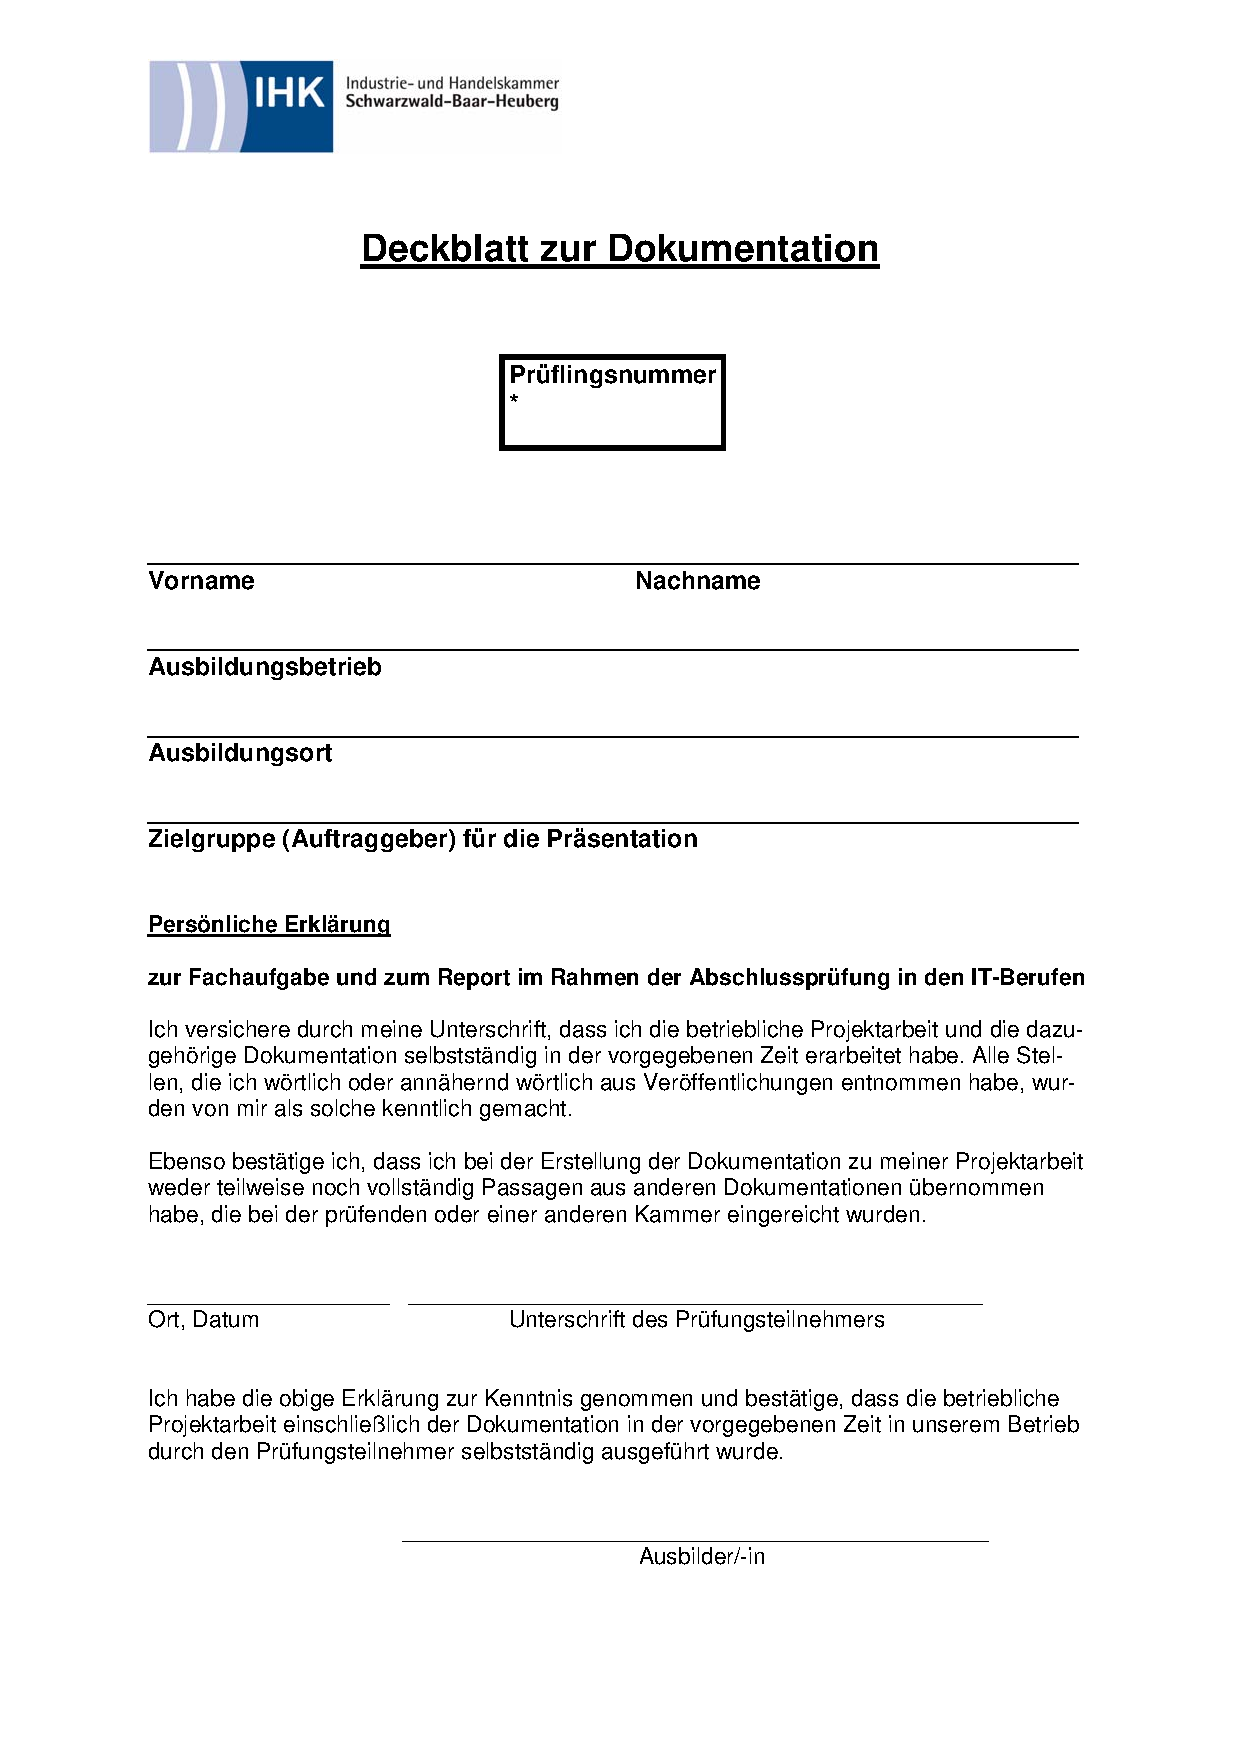
\includegraphics[graphicx]{content/Frontpage.pdf}

\phantomsection
% !TEX root = Index.tex
\clearpage

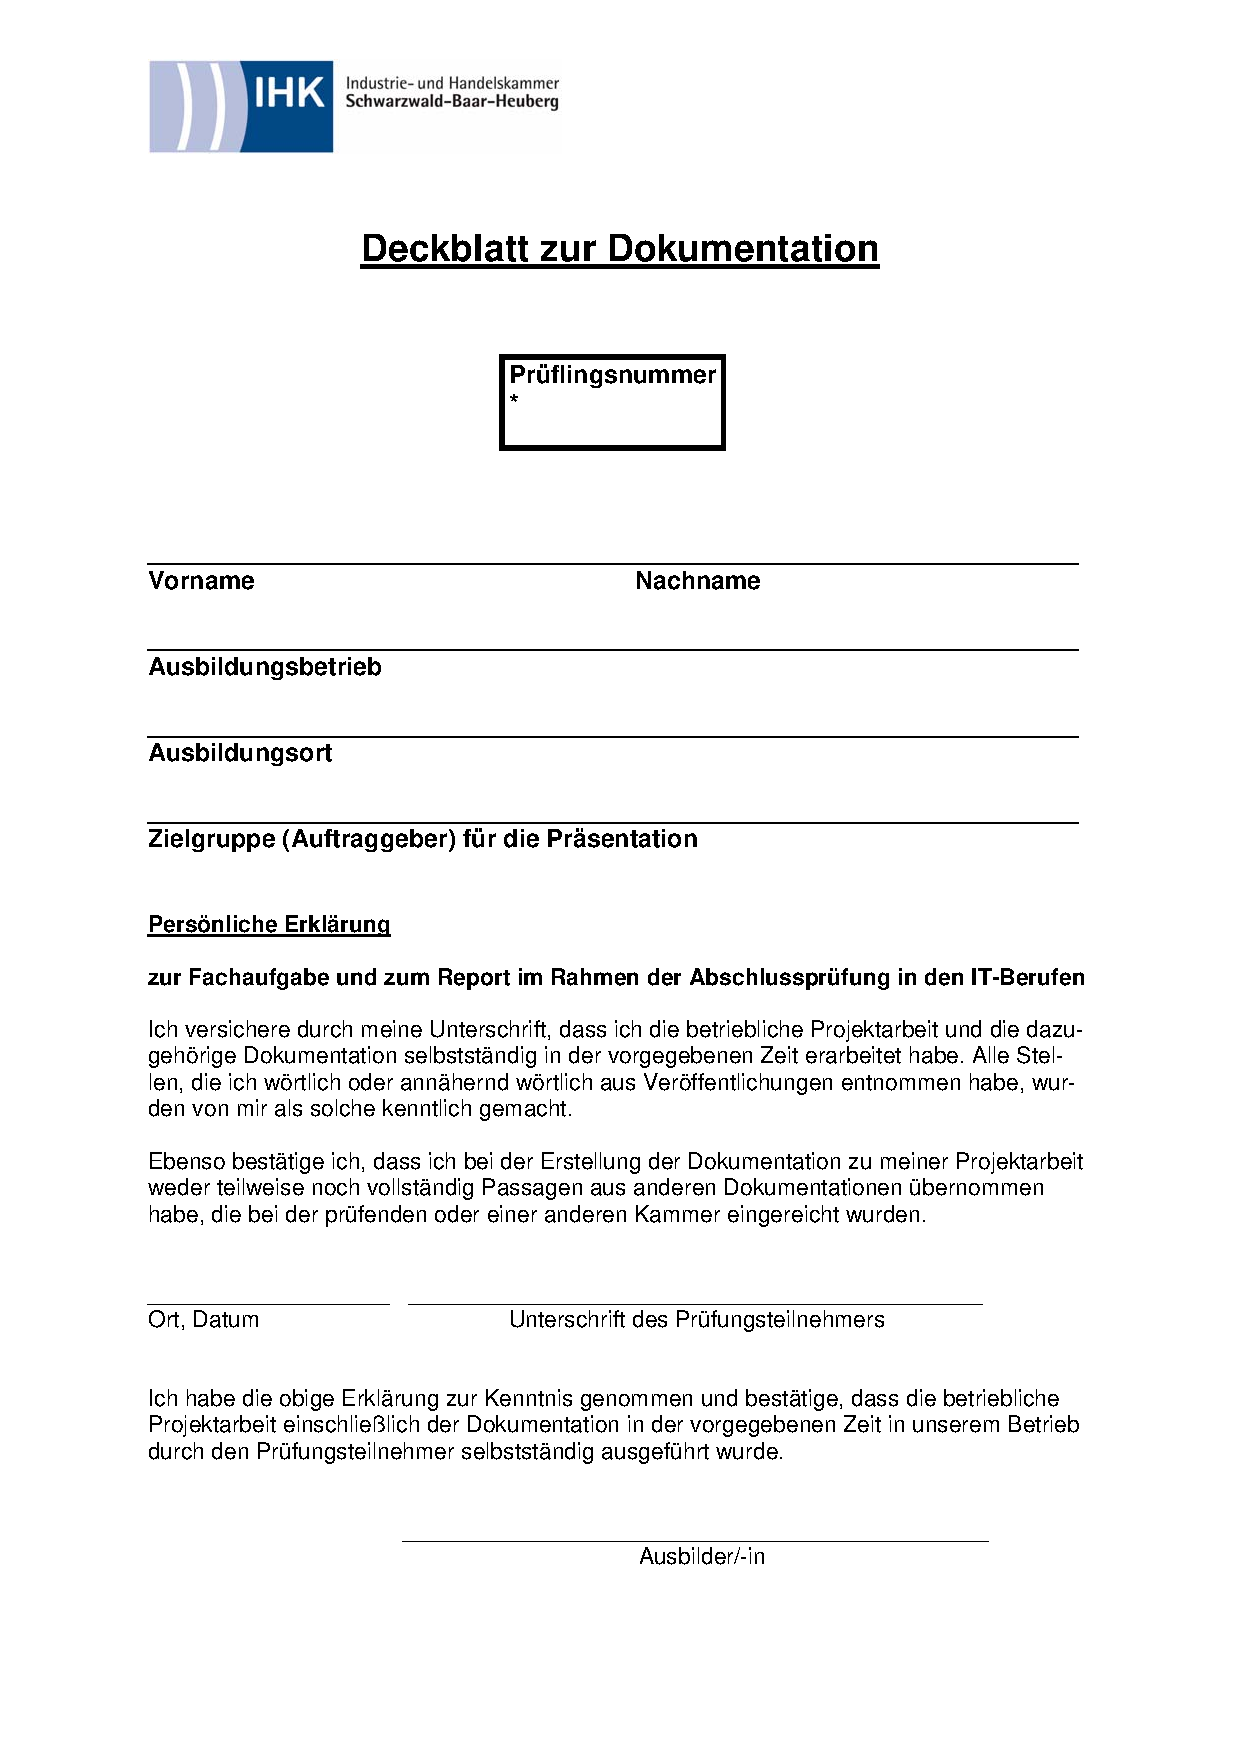
\includepdf{content/Frontpage.pdf}



\includepdf[pages={1-7}]{content/Antrag.pdf}


\thispagestyle{plain}
\pdfbookmark[1]{Deckblatt}{deckblatt}
% !TEX root = Index.tex
\begin{titlepage}

\begin{center}

\includegraphics[scale=0.15]{img/ihk-logo.jpg}\\[1ex]
\Large{Abschlussprüfung \pruefungstermin}\\[3ex]

\Large{\ausbildungsberuf}\\
\LARGE{\betreff}\\[4ex]

\huge{\textbf{\titel}}\\[1.5ex]
\Large{\textbf{\untertitel}}\\[4ex]

\normalsize
Abgabetermin: \abgabeOrt, den \abgabeTermin\\[3em]
\textbf{Prüfungsbewerber:}\\
\autorName\\
\autorAnschrift\\
\autorOrt\\[5ex]

\includegraphics[scale=0.2]{\betriebLogoBig}\\[2ex]
\textbf{Ausbildungsbetrieb:}\\
\betriebName\\
\betriebAnschrift\\
\betriebOrt\\[5em]
\end{center}

\small
\noindent
Dieses Werk einschließlich seiner Teile ist \textbf{urheberrechtlich geschützt}.
Jede Verwertung außerhalb der engen Grenzen des Urheberrechtgesetzes ist ohne
Zustimmung des Autors unzulässig und strafbar. Das gilt insbesondere für
Vervielfältigungen, Übersetzungen, Mikroverfilmungen sowie die Einspeicherung
und Verarbeitung in elektronischen Systemen.

\end{titlepage}
\cleardoublepage

% Preface --------------------------------------------------------------------
\phantomsection
\pagenumbering{Roman}
\pdfbookmark[1]{Inhaltsverzeichnis}{inhalt}
\tableofcontents
\cleardoublepage

\newcommand{\abkvz}{Abkürzungsverzeichnis}
\renewcommand{\nomname}{\abkvz}
\section*{\abkvz}
\markboth{\abkvz}{\abkvz}
\addcontentsline{toc}{section}{\abkvz}
% !TEX root = Index.tex

% Die Option (in den eckigen Klammern) enthält das längste Label oder
% einen Platzhalter der die Breite der linken Spalte bestimmt.
\begin{acronym}[WWWWW]
    % Programme
    \acro{IDE}{Integrated Development Environment}
    \acro{CMD}{Eingabeaufforderung}
	\acro{Node}[NodeJS]{JavaScript Interpreter}
	\acro{IIS}{Microsoft Internet Information Services}
	
    % IT Fachwörter
    \acro{UI}{Oberfläche}
	\acro{API}{Application Programming Interface}
	\acro{MVC}[MVC]{Model View Controller}
	\acro{ORM}{Object-Relational Mapping}
	\acro{UML}{Unified Modeling Language}
	\acro{ERM}{En\-ti\-ty-Re\-la\-tion\-ship-Mo\-dell}
	
	% Programmier-, Script-, Deklerationssprachen 
	\acro{CSS}{Cascading Style Sheets}
	\acro{HTML}{Hypertext Markup Language}\acused{HTML}
	\acro{.NET}{Microsoft .NET}
	\acro{CS}[C\#]{C-Sharp}
	\acro{JS}{JavaScript}
	
	% Frameworks
	\acro{React}[ReactJS]{React JavaScript}
	\acro{ASP}[ASP.NET]{Active Server Pages .NET}
	\acro{REST}{Representational State Transfer}
	\acro{ODBC}{Open Database Connectivity}
	
	% Datenverarbeitung
	\acro{XML}{Extensible Markup Language}
	\acro{SQL}{Structured Query Language}
	\acro{JSON}{JavaScript Object Notation}
	
	% Fachwörter (Allgemein)
	\acro{ERP}{Enterprise Resource Planning}
	\acro{CRM}{Customer Relationship Management}
\end{acronym}
\clearpage

\phantomsection
\listoffigures
\cleardoublepage

\phantomsection
\listoftables
\cleardoublepage

\phantomsection
\lstlistoflistings
\cleardoublepage

% Inhalt ---------------------------------------------------------------------
\pagenumbering{arabic}
% !TEX root = Index.tex
% !TEX root = ../Index.tex
\section{Einleitung}
\label{sec:Einleitung}


\subsection{Projektumfeld} 
\label{sec:Projektumfeld}
Das Projekt wird von Christopher Mogler in der Firma Weiss GmbH Softwarelösungen
entwickelt. Sie wurde 1975 von Rolf Weiss mit Hauptsitz in Schiltach gegründet. Zu den ersten
Anfängen der Firma wurde für mittelständische Unternehmen Auftragsprogrammierungen auf
IBM-Systemen durchgeführt. Im Jahre 1985 wurde die Produktpalette auf \acsu{ERP}-Systeme, für
mittelständische und größere Handels bzw. Industrieunternehmen, erweitert. \\
Die Geschäftsleitung wurde 1998 von Martin Lauble übernommen. Ab dem Jahr 2002 wurde der
Schwerpunkt der Software auf das Produkt PowerWeiss für Windows gelegt, welches als
\acsu{CRM}-System für Handel, Industrie und Versicherungsagenturen genutzt werden kann.

\subsection{Projektziel} 
\label{sec:Projektziel}
Die Firma hat für viele Zusatz Module dazugehörige Dienste. Diese müssen installiert und konfiguriert werden. \\
Der Support muss sich auf die Kunden-Server drauf schalten und danach die Dienste manuell installieren und konfigurieren. Ziel ist es die Installation, Aktualisierung und Deinstallation zu automatisieren.
Deshalb soll ein Dienst programmiert werden, was die anderen Dienste automatisch verwaltet. 
Über eine Oberfläche kann die Firma Weiss, Dienste installieren, konfigurieren, aktualisieren und deinstallieren. Der Dienst auf dem Kunden-Server holt sich die aktuellen Daten über eine \acsu{REST}-\acsu{API} ab. \\
Und gleicht die Dienste mit den Daten der \acsu{API} ab. 
Bei einer Installation sollen die Dateien heruntergeladen werden. Danach werden die Dateien in ein Verzeichnis gespeichert. Die Dienste werden über die Windows-\acsu{API} per \acsu{CS} installiert. Die Dienste werden direkt gestartet.
Bei einer Aktualisierung werden die ausgewählten Dienste gestoppt. Die Dateien werden mit den aktuellen Dateien überschrieben. Danach wird der Dienst wieder gestartet.
Wenn Dienste deinstalliert werden sollen, werden die Dienste gestoppt und über die Windows-\acsu{API} vom Dienst-Verzeichnis entfernt. Die Dateien werden nicht gelöscht, um Fehler vorzubeugen.
\subsection{Projektbegründung} 
\label{sec:Projektbegruendung}
Um Dienste zu installieren muss sich ein Mitarbeiter, der Firma Weiss, auf den Server drauf schalten. 
Die aktuellen Dateien der Dienste kopieren und mit dem Windows bereitgestellten Programm "InstallUtil" installieren. Da "InstallUtil" nur über eine \acsu{CMD} verwendet werden kann, ist es sehr fehleranfällig. \\
Die manuelle Installation ist sehr Zeit aufwendig, deshalb ist eine Automatisierung sehr sinnvoll.
Mit einer Automatisierung werden Dienste per Knopfdruck In-, aktuali- und Deinstalliert oder konfiguriert, ohne das ein Mitarbeiter sich auf einen Server Zugriff verschaffen muss. 

\subsection{Projektschnittstellen} 
\label{sec:Projektschnittstellen}
\begin{itemize}
	\item Mit welchen anderen Systemen interagiert die Anwendung (technische Schnittstellen)?
	\item Wer genehmigt das Projekt \bzw stellt Mittel zur Verfügung? 
	\item Wer sind die Benutzer der Anwendung?
	\item Wem muss das Ergebnis präsentiert werden?
\end{itemize}
Für die Datenspeicherung wird eine SQL-Anywhere-Datenbank verwendet. Der Zugriff auf diese Datenbank, wird über \acsu{ODBC} realisiert. \\
\acsu{UI} und \acsu{REST} werden als Web Applikation bereitgestellt, diese wird über \acsu{ASP} verwaltet. Um \acsu{ASP} zu verwenden wird ein \acsu{IIS}-Dienst von Windows benötigt. \\
Um Windows-Dienste verwalten zu können, wird auf die Windows-\acsu{API} zugegriffen, über die AdvAPI32 Bibliothek. \\
\acsu{UI} verwendet \acsu{React} als Framework und \acsu{Node} zur verwaltung von \acsu{React}. 
\\
Das Projekt wurde durch Herrn Richter genehmigt, der Abteilungsleiter der Entwicklung – bei der Firma Weiss. Die Endnutzer sind die Mitarbeiter der Firma Weiss, die geschult werden durch den Autor und eine Anwenderdokumentation erhalten. \\

\subsection{Projektabgrenzung[TODO]} 
\label{sec:Projektabgrenzung}
\begin{itemize}
	\item Was ist explizit nicht Teil des Projekts (\insb bei Teilprojekten)?
\end{itemize}

% !TEX root = ../Projektdokumentation.tex
\section{Projektplanung} 
\label{sec:Projektplanung}


\subsection{Projektphasen}
\label{sec:Projektphasen}

Das Projekt wurde vom 20. April bis 05. Mai realisiert. Der Arbeitstag wurde in diesem Zeitraum in sieben Stunden für das Projekt und eine Stunde für andere Themen aufgeteilt. Andere Themen sind \zB Fehlerbehebung, Support und Telefondienst. \*

Tabelle~\ref{tab:Zeitplanung} zeigt die grobe Zeitplanung.
\tabelle{Zeitplanung}{tab:Zeitplanung}{TimetableShort} 
Eine detaillierte Zeitplanung findet sich im \Anhang{app:timer}.

\subsection{Abweichungen vom Projektantrag}
\label{sec:AbweichungenProjektantrag}

Im Projektantrag wurde eine Offline Installation aufgeführt. Diese wurde aber durch die Leitung als nicht mehr relevant angesehen. Daher ist diese nicht etabliert worden. \\
\\
Bei einer Versionsänderung werden die Dateien komplett mit den neuen überschrieben. Das hat den Vorteil: weniger Quellcode für die Versionsprüfung und verringerte Fehler, bei einer falschen Validierung. Die Performance wird nicht beeinträchtigt, weil die Dienste nicht groß sind und selten viele einzelne Dateien vorweisen. 

\subsection{Ressourcenplanung}
\label{sec:Ressourcenplanung}

Entwickelt wurde in Schiltach im Büro des Entwicklerteam 1.
Von der Firma Weiss wurde die benötigten Ressourcen Hard- und Software bereitgestellt. \\
\\
Um Kosten gering wie möglich zu halten, wurde auf Software zurückgegriffen die frei zur Verfügung steht oder bereits Lizenzen im Unternehmen vorhanden waren. Hier ist eine Liste der verwendeten Anwendungen:
\begin{itemize}
    \item Visual Studio 2019    (\acsu{IDE})
    \item Windows 10            (Betriebssystem)
    \item SQL Anywhere          (\acsu{DBMS})
    \item Interactive SQL       (\acsu{SQL} Editor mit integrierter Datenbank Schnittstelle)
    \item SQL Central           (Administrations Tool für SQL Anywhere)
    \item .NET Framework / Core (Runtime für \acsu{CS})
    \item ReactJS               (Frontend-\acsu{JS}-Framework)
    \item Bootstrap             (Frontend-\acsu{CSS}-Framework)
    \item NodeJS                (Runtime für \acsu{JS})
\end{itemize}

Als organisatorische Hilfe wurde Herr Oehler zur Verfügung gestellt, für den Autor.

\subsection{Entwicklungsprozess}
\label{sec:Entwicklungsprozess}

Da die einzelnen Programme nicht sehr aufwendig waren, wurde das erweiterte Wasserfallmodell eingesetzt.\\
\\
Die Implementierungsphase wurde in iterativen Zyklen durchgeführt. Ferner ist zu beachten, dass die einzelnen Teile komplett entwickelt wurden. Jedes Teilprojekt ist nach der Fertigstellung getestet worden, um neue oder vorhandene Funktionen auf Fehler zu prüfen.



%% !TEX root = ../Index.tex
\section{Analysephase} 
\label{sec:Analysephase}


\subsection{Ist-Analyse} 
\label{sec:IstAnalyse}

Wenn ein Kunden-System angepasst werden muss, benötigt der Mitarbeiter der Firma Weiss Zugriff auf dieses System. Er muss einen Remotezugriff aufbauen, oft wird die Anwendung TeamViewer dafür verwendet.\\
Es kann vorkommen, dass die Fernwartung nicht durchgeführt werden kann. Die Ursache können sein: Das die entsprechende Software nicht ausgeführt wird, auch kann es an aktuelle Probleme eines Internetproviders liegen, bestimmte Kundenserver können nur über einen Client-Rechner vom Kunden erreicht werden, selten müssen sich Mitarbeiter den Zugriff über den Kunden freischalten lassen.\\
Es werden Systeme Eingriffe durchgeführt, dadurch werden administrative Rechte benötigt. \\
\\
Bei einer Installation eines Dienstes wird der Zugriff auf den Kundenserver benötigt.\\
Hat ein Mitarbeiter Zugriff auf den Kundenserver, so müssen die Dateien für die Dienste auf den Server kopiert werden.
Sind die Dateien auf das System kopiert, so kann der Mitarbeiter die Dateien aufbereiten für die Installation. Der Mitarbeiter kann frei entscheiden, wo die Dienste installiert werden. Um einen Dienst installieren zu können wird das InstallUtil-Tool, was von Windows bereitgestellt wird, verwendet. Dieses Tool kann nur über eine Eingabeaufforderung angesteuert werden. Ferner ist zu beachten, dass eine fehlerhafte Installation, aus der Log, nicht direkt ersichtlich ist. Sollte die Installation erfolgreich sein, muss die Konfigurationsdatei angepasst werden. Im Anschluss muss der Mitarbeiter den Dienst zusätzlich starten. Der Dienst sollte nach dem Starten geprüft werden, ob Fehler auftauchen: Status des Dienstes in der Diensteverwaltung von Windows, Ereignisanzeige oder Log-Datei. Nachdem der Dienst installiert und geprüft wurde, kann der Fernzugriff beendet werden.\\
\\
Muss ein Dienst angepasst werden, so führt der Mitarbeiter eine Fernwartung durch, um Zugriff auf das Kundensystem zu bekommen. Bevor ein Dienst angepasst werden kann, muss dieser zuvor gestoppt werden. Das bei der Installation der Pfad frei gewählt werden kann, kann es vorkommen, dass die Installationspfade der Dienste nicht direkt gefunden werden.\\
Sollte nur die Konfiguration angepasst werden, wird diese über den vorhandenen Text-Editor beim Kunden bearbeitet und gespeichert.\\
Bei einer Versionsänderung müssen die passenden Version Dateien gesucht und auf das System hochgeladen werden. Die Dateien haben keinen einheitlichen Ablageort. Um die Versionsänderung durchzuführen, werden die Dateien mit den neuen überschrieben. Es kann vorkommen, dass die Konfigurationsdatei mit überschrieben wird. \\
Nach der Anpassung kann der Dienst erneut gestartet werden. Wie bei der Installation sollte nach dem Starten der Dienst noch zusätzlich geprüft werden.\\
\\
Sollte ein Dienst nicht mehr im Gebrauch sein, so kann dieser aus dem Kundensystem entfernt werden. Dazu benötigt der Mitarbeiter Zugriff auf das System, wo der Dienst installiert ist. Um Dienste aus dem Dienst-Pool von Windows entfernen zu können, wird das gleiche Tool, wie bei der Installation verwendet. Auch hier ist zu beachten, dass die Log-Ausgabe nicht direkt darauf hinweist, dass ein Fehler entstanden ist. InstallUtil übernimmt das Stoppen des Dienstes, bei der Deinstallation. Die Dienst-Dateien müssen nicht entfernt werden. Sollen die Dateien entfernt werden, so muss der Mitarbeiter den Installations-Pfad des Dienstes herausfinden und die Dateien löschen.

\subsection{Wirtschaftlichkeitsanalyse}
\label{sec:Wirtschaftlichkeitsanalyse}

Sollte ein Mitarbeiter keinen direkten Zugriff auf einen Server bekommen, so wird hier viel Zeit benötigt für die Kommunikation und Organisation mit dem Kunden. Wenn der Verwaltungsdienst bereits beim Kunden installiert ist, wird kein Fernzugriff mehr benötigt. Der Dienst kann komplett autonom die Dienste verwaltet. \\
\\
Version Dateien für Dienste müssen gesucht werden, da es keinen standardisierten Ablageort gibt. Durch die Oberfläche sind alle Dienste tabellarisch aufgelistet. Die Entwickler laden über die Oberfläche aktuelle Versionen mit dazugehöriger Konfiguration hoch. Hier ergibt sich ein einheitlicher Ablageort. \\
\\
Beim Installieren und Deinstallieren von Diensten, wird InstallUtil benötigt. Dieses Tool kann nur über eine Eingabeaufforderung verwendet werden. Es ist Fehleranfälliger und Fehler werden in der Log nicht direkt ersichtlich. Durch die Oberfläche können Dienste per Knopfdruck installiert oder wieder entfernt werden.
\\
Es kann Zeit gespart und Fehler minimiert werden. Man kann Abläufe besser kontrolliert und steuern.

\subsubsection{\gqq{Make or Buy}-Entscheidung}
\label{sec:MakeOrBuyEntscheidung}

Es gibt Anwendungen die Dienste verwalten und Statusmeldung zurückliefern können. Aus wirtschaftlicher Sicht ist trotzdem die “Make”-Methode gewählt worden. Die Anwendungen haben zu viele andere Funktionen, die nicht verwendet werden. Was es dadurch nicht wirtschaftlich macht, wenn für die meisten Funktionen bezahlt wird, aber diese nicht verwendet werden.

\subsubsection{Projektkosten}
\label{sec:Projektkosten}

Die Kosten für die Durchführung des Projekts setzen sich sowohl aus Personal-, als auch aus Ressourcenkosten zusammen. Der Autor verdient als Auszubildender \eur{950} im Monat. 

\begin{eqnarray}
8 \mbox{ h/Tag} \cdot 220 \mbox{ Tage/Jahr} = 1.760 \mbox{ h/Jahr}\\
\eur{950}\mbox{/Monat} \cdot 12 \mbox{ Monate/Jahr} = \eur{11.400} \mbox{/Jahr}\\
\frac{\eur{11.400} \mbox{/Jahr}}{1.760 \mbox{ h/Jahr}} \approx \eur{6,477}\mbox{/h}
\end{eqnarray}

Es ergibt sich also ein Stundenlohn von \eur{6,477}. 
Die Durchführungszeit des Projekts beträgt 70 Stunden. Für die Nutzung von Ressourcen\footnote{Räumlichkeiten, Arbeitsplatzrechner etc.} wird 
ein pauschaler Stundensatz von \eur{15} angenommen. Für die anderen Mitarbeiter wird pauschal ein Stundenlohn von \eur{30} angenommen. 
Eine Aufstellung der Kosten befindet sich in Tabelle~\ref{tab:Kostenaufstellung} und sie betragen insgesamt \eur{2.663,39}.
\tabelle{Kostenaufstellung}{tab:Kostenaufstellung}{Kostenaufstellung.tex}

\subsubsection{Amortisationsdauer}
\label{sec:Amortisationsdauer}

Bei einer Zeiteinsparung von 30 Minuten am Tag für jeden der 10 Anwender und 220 Arbeitstagen im Jahr ergibt sich eine gesamte Zeiteinsparung von 
\begin{eqnarray}
10 \cdot 220 \mbox{ Tage/Jahr} \cdot 30 \mbox{ min/Tag} = 66.000 \mbox{ min/Jahr} \approx 1.100 \mbox{ h/Jahr} 
\end{eqnarray}

Dadurch ergibt sich eine jährliche Einsparung von 
\begin{eqnarray}
1.100 \mbox{h} \cdot \eur{(30 + 15)}{\mbox{/h}} = \eur{49.500}
\end{eqnarray}

Die Amortisationszeit beträgt also $\frac{\eur{2.663,39}}{\eur{49.500}\mbox{/Jahr}} \approx 0,054 \mbox{ Jahre} \approx 2,4 \mbox{ Wochen}$.

Das Projekt hat sich also innerhalb von zwei bis drei Wochen amortisiert. 

\subsection{Anwendungsfälle}
\label{sec:Anwendungsfaelle}

\subsubsection{Installation}
\label{sec:Fall_Installation}

Wenn beim Kunden ein Dienst installiert werden soll, wird über eine Oberfläche der Dienst mit der Version ausgewählt. Die Oberfläche zwingt die Anpassung der Konfiguration. Beim Speichern werden die Daten in die Datenbank gespeichert. Der Dienst beim Kunden selektiert die Daten und installiert automatisch diesen Dienst mit der gelieferten Konfigurationsdatei.

\subsubsection{Versionsänderung}
\label{sec:Fall_Update}

Sollte beim Kunden eine neue oder andere Version installiert sein, wird dies wieder über die Oberfläche gesteuert. Die Konfigurationsdatei wird mit der neuen Konfiguration ausgetauscht. Alle Änderungen werden wieder in die Datenbank der Firma Weiss gespeichert. Über die Web-Schnittstelle bekommt der Verwaltungsdienst die Änderungen mitgeteilt und aktualisiert den Dienst. \\
Beim ändern der Dateien von einem Dienst muss der Dienst gestoppt werden, dies wird vom Verwaltungsdienst übernommen. Und bei erfolgreicher Installation wieder gestartet. 

\subsubsection{Anpassung}
\label{sec:Fall_Anpassung}

Über die Oberfläche wird die Konfiguration angepasst, wenn diese Fehlerhafte oder veraltete Daten enthält. Beim speichern werden die änderungen in die Datenbank der Firma Weiss gespeichert. Der Dienst bekommt die Änderung mit und überschreibt die aktuelle Konfigurationsdatei. \\
Der Dienst wird davor gestoppt und nach dem Austausch wieder gestartet. 

\subsubsection{Deinstallation}
\label{sec:Fall_Deinstallation}

Bei einer Deinstallation wird der Dienst über eine Oberfläche entfernt. Der Status in der Datenbank wird zu \Datentyp{REMOVE} geändert. Beim Kunden wird der Dienst gestoppt und aus dem Dienst-Pool von Windows entfernt.

\subsubsection{Statusmeldung}
\label{sec:Fall_Status}

Status und Zustände der aktuellen Dienste werden regelmäßig überliefert und in die Datenbank gespeichert. Über die Oberfläche kann in der Kundenansicht die Stati der Dienste gesehen werden. 



%% !TEX root = ../Index.tex
\section{Entwurfsphase} 
\label{sec:Entwurfsphase}

\subsection{Zielplattform}
\label{sec:Zielplattform}

Für \acsu{DBMS} wurde SQL-Anywhere verwendet. Durch die Standardisierung der Firma Weiss, ist es bereit bei jedem Kunden installiert. \\
Der Verwaltungsdienst und die Web-Anwendung wurden in \acsu{CS} programmiert. Einer der standardisierten Programmiersprachen in der Firma Weiss ist \acsu{CS}. Daher besitzen alle System von Kunden und der Firma Weiss die benötigte Software um die Applikationen ausführen zu können. \\
Die Web-Anwendungen verwenden als Background Framework \acsu{ASP}, dadurch wird können \acsu{HTTP} Anforderungen einfacher bearbeitet und zurückgegeben werden. \\
\\
Die Oberfläche verwendet als Frontend Framework ReactJS. Da ReactJS auf \acsu{MVC}-Paradigma aufbaut, wird viel rekursiver Code gespart und hat zu einem großen Zeitersparnis geführt.  \\
Ferner ist zu beachten, dass die Oberfläche als Webanwendung realisiert wurde. Dadurch sinkt die Wartungsarbeit für einzelne Rechner und zudem steigt die Benutzerfreundlichkeit, keine Zusatzsoftware installiert werden muss. Updates sind für den Endbenutzer nicht relevant, da die Versionsänderung Serverseitig stattfindet. Man ist als Web-Anwendung nicht System gebunden, was dazu führt das man mit jedem Browser fähigen Endgerät die Dienste verwalten und steuern kann. Das Gerät sollte aber einen aktuellen Browser verwenden. \\
Um bestimmte Funktionen von ReactJS steuern zu können, muss Serverseitig eine NodeJS Anwendung laufen. \\
\\
Die \acsu{API} wurde auf den \acsu{REST}-Standard aufbaut. Aus diesem Grund wurde die Anwendung als Webapplikation realisiert. Es gibt unterschiedliche \acsu{REST}-Methoden, diese können problemlos mit \acsu{HTTP}-Methoden überlagert werden.\\
\\
Der Verwaltungsdienst wurde als Windows-Dienst realisiert. Die Anwendung läuft im Hintergrund und wird daher als Dienst programmiert. Um Dienste verwalten und steuern zu können, wird auf die Windows-\acsu{API} zugegriffen. Als Bibliothek wird die AdvAPI32 verwendet. Diese wird von Windows bereitgestellt. \\
Alle Kunden-Systeme laufen auf Windows-Betriebssystemen, daher muss nicht zwingend Systemübergreifend programmiert werden.

\subsection{Architekturdesign}
\label{sec:Architekturdesign}

Die Webanwendung wurde mit \acsu{ASP} realisiert. \acsu{ASP} ist ein Framework für \acsu{CS}, um die Kommunikation über \acsu{HTTP} zu vereinfachen. Es ist Open-Source und kann frei genutzt werden, zudem wird aktiv daran weiterentwickelt und ist sehr Performant. \\
\\
Für die Oberfläche wurde ReactJS und Bootstrap verwendet. \\
ReactJS ist ein Framework was oft für Single-Page-Applikationen verwendet wird. Das bedeutet, dass eine komplette Anwendung nur über eine \acsu{HTML}-Seite funktioniert. Um das Realisieren zu können wird die Seite in Komponenten aufgeteilt. Durch \acsu{JSX} wird es ermöglicht in JavaScript \acsu{HTML}-Code zu schreiben. Komponenten können daher aus JavaScript und \acsu{HTML} bestehen. Durch Komponenten wird viel rekursiver Code gespart, das hat den Grund, dass Komponenten mehrfach eingesetzt werden können. \\
\\
Der Dienst wird als Windows-Dienst realisiert. Es hat den Grund um die Anwendung von Windows-Dienst-Pool verwalten zu lassen. Das hat den Vorteil, dass die Anwendung komplett im Hintergrund laufen kann. \\
\\
Das \acsu{MVC}-Paradigma  unterteilt die Anwendung in drei Bereiche. Model, repräsentiert die Daten; View, zeigt die Daten an; Controller, verbindet Model mit der View. Die Zielsetzung ist es den Quellcode zu vereinfachen und die Wiederverwendbarkeit zu steigern.


\subsection{Entwurf der Benutzeroberfläche}
\label{sec:Benutzeroberflaeche} 

Im Anhang sind die erstellten Konzepte Designs für die Oberfläche. Diese wurden mit dem Mockup-Programm Pencil erstellt. Die Designs konzentrierten sich auf Benutzerfreundlichkeit, weil die Oberfläche nur für interne zugänglich ist. Ferner wurde auf Corporate Design verzichtet.\\
Aus Zeitgründen wurde auf die Optimierung der Oberfläche für Mobile Endgeräte verzichtet. 

\subsection{Datenmodell}
\label{sec:Datenmodell}

Die endgültigen Tabellen und Datenstrukturen wurde in einem Tabellenmodell konzeptioniert. Zeitgleich wurden die Relationen, mit deren Kardinalitäten, gezeichnet. \\
Im \Anhang{app:database_table} finden sich die Konzeptionierten Modelle, mit deren Entitäten.

\subsection{Geschäftslogik}
\label{sec:Geschaeftslogik}

Die Aktivitätsdiagramme wurden mit ARIS Express erstellt. Das Aktivitätsdiagramm  wurde im \Anhang{app:useCase_controll} beigefügt. Das Diagramm zeigt den Ablauf für die Oberfläche und Dienstprüfung. 



%% !TEX root = ../Projektdokumentation.tex
\section{Implementierungsphase} 
\label{sec:Implementierungsphase}

\subsection{Implementierung der Datenstrukturen}
\label{sec:ImplementierungDatenstrukturen}

Die Tabellen wurden mit hilfe von SQL Central erstellt. Der Autor musste die aufwendigen \acsu{SQL}-Scripts nicht selber schreiben. \\
Die \acsu{SQL}-Skripte können über SQL Central generiert werden. Zum Erstellen der Tabellen auf der Datenbank, müssen nur die generierten Skripte auf der Datenbank ausgeführt werden. 


\subsection{Implementierung der Benutzeroberfläche}
\label{sec:ImplementierungBenutzeroberflaeche}

Die Oberfläche wurde als Webapplikation und auf Basis einer Single-Page-Anwendung realisiert. Als Frontend Framework wurde ReactJS verwendet. \\
ReactJS Seiten werden in Komponenten aufgeteilt, um Code und vor allem rekursiven Code zu sparen. \\
Komponenten bestehen aus \acsu{JSX}-Dateien. \acsu{JSX} ist eine von React entwickeltes Format. Es ermöglicht in JavaScript \acsu{XML}/\acsu{HTML} Code zu verwenden. Komponenten können auch mehrfach verwendet werden.\\
Als Frontend-\acsu{CSS}-Framework wurde Bootstrap verwendet. \\
Teile der Seite sind im \Anhang{app:view_real}, als Screenshots beigefügt.


\subsection{Implementierung der Geschäftslogik}
\label{sec:ImplementierungGeschaeftslogik}

Um die Dienste installieren zu können wurde die Windows-\acsu{API} angesprochen. Dies wurde mit der AdvAPI32 Bibliothek durchgeführt. Bevor diese verwendet werden kann, muss die bestimmten Funktion der Bibliothek importiert werden. Siehe \Anhang{app:sourceCode} erstes Abbild. \\
Um auf den Dienst-Pool zugreifen zu können, wird der ServiceControll-Manager von Windows geöffnet. Dadurch bekommt der Dienst die Berechtigung Dienste zu Verwalten. \\
Wenn ein Dienst deinstalliert werden soll, wird der Dienst gestoppt (wird von der Bibliothek übernommen) und vom Dienst-Pool entfernt.
Sollte ein Dienst hinzugefügt werden, wird der Dienstname, der Pfad der Dienst-Anwendung und über welchen Benutzer der Dienst gestartet werden soll angegeben. Nach dem Hinzufügen wird die Rückmeldung der Funktion geprüft, ob Fehler entstanden sind.\\ Wenn nicht, wird der Dienst gestartet und beim erfolgreichen Start wird die Installation als abgeschlossen angesehen.

%% !TEX root = ../Index.tex
\section{Abnahmephase} 
\label{sec:Abnahmephase}

%\begin{itemize}
%	\item Welche Tests (\zB Unit-, Integrations-, Systemtests) wurden durchgeführt und welche Ergebnisse haben sie geliefert (\zB Logs von Unit Tests, Testprotokolle der Anwender)?
%	\item Wurde die Anwendung offiziell abgenommen?
%\end{itemize}

%\paragraph{Beispiel}
%Ein Auszug eines Unit Tests befindet sich im \Anhang{app:Test}. Dort ist auch der Aufruf des Tests auf der Konsole des Webservers zu sehen.

%% !TEX root = ../Projektdokumentation.tex
\section{Einführungsphase}
\label{sec:Einfuehrungsphase}

\subsection{Anwendungen}
\label{sec:programs_install}

\subsubsection{Oberfläche / \acsu{UI}}
\label{sec:UI}

Die Oberfläche wurde auf dem Cloud-Server der Firma Weiss hochgeladen. Auf diesen Cloud-Server läuft ein Windows-Betriebssystem mit der \acsu{IIS}-Applikation. \\
Die Webanwendungen kann nur aus dem lokalen Netz abgerufen werden, um Unautorisierte Zugriffe zu verhindern. Um Außerhalb der Firma zugreifen zu können, wird ein \acsu{VPN}-Tunnel benötigt. 

\subsubsection{API}
\label{sec:API}

Die \acsu{API} läuft wie die Oberfläche auf dem Cloud-Server der Firma Weiss. Die API ist aus dem öffentlichen Netz erreichbar, da die Daten nur über einen \acsu{SHA}-512 Token freigegeben werden. 

\subsubsection{Verwaltungsdienst}
\label{sec:Service}

Um die Mitarbeiter zu Schulen, wurde auf einem Testgerät der Firma Weiss dieser Verwaltungsdienst installiert. Dieser ist mit einem Testkunde verknüpft.\\
\\
In der Schulung wurden die Dienste auf ausgewählten Kunden-Systeme installiert und ausgeführt.\\
\\
Dadurch das der Dienst sich selbst installieren kann, muss dieser nur ausgeführt werden. Davor muss die Konfiguration angepasst werden: Authentifizierung Token, Datenbank \acsu{ODBC} Daten, Filestore wo die Dienste installiert werden soll. 

\subsection{Schulung}
\label{sec:Schulung}

Die Mitarbeiter wurden in einer 2,5 stündigen Schulungsveranstaltung geschult. Es wurde die Oberfläche präsentiert und erklärt. Danach ist auf die Installation des Verwaltungsdienst eingegangen worden. \\
Die Mitarbeiter mussten selbst auf Kundensysteme den Verwaltungsdienst installieren und konfigurieren. \\
In den letzten 10min ist man auf Fragen und Anregungen eingegangen.

%% !TEX root = ../Projektdokumentation.tex
\section{Dokumentation}
\label{sec:Dokumentation}

%% !TEX root = ../Projektdokumentation.tex
\section{Fazit} 
\label{sec:Fazit}

\subsection{Soll-/Ist-Vergleich}
\label{sec:SollIstVergleich}

Das Projektziel wurde erfüllt. Es ist möglich Dienste direkt über die Webapplikation zu steuern. \\
Der Status der Dienste wird rückgemeldet, ob diese Laufen, gestoppt sind, etc.

\tabelle{Zeitplanung Soll-/Ist-Vergleich}{tab:ZeitplanungSollIst}{SI_Timetable}

\subsection{Lessons Learned}
\label{sec:LessonsLearned}

Der Autor konnte lernen wie eine richtige \acsu{REST}-Anwendung aufgebaut wird. Mit den \acsu{HTTP}-Statusen und Authenfizierungstokens. Auch wie man über \acsu{CS} auf die Windows-\acsu{API} zugreifen kann und darüber Windows-Dienste installieren kann. Wie man \acsu{DLL}s in \acsu{CS} einbindet und die jeweiligen Funktionen importiert. \\
Wie man von Grund auf eine Webapplikation entwickelt und diese den Endbenutzern erklärt und schult. \\
Aus einer Idee ein komplett strukturiertes Projekt mit Dokumentation, Zeitmanagement und Ressourcenplanung.


\subsection{Ausblick}
\label{sec:Ausblick}
Der Autor wird nach der Ausbildung die Firma Weiss verlassen, das Produkt wird an das EntwicklerTeam-1 übergeben.
Geplante Erweiterungen sind Fernsteuerung der Dienste: z. B. Stoppen, Starten, Neu Starten.
\clearpage

% Anhang ---------------------------------------------------------------------
\appendix
\pagenumbering{roman}
% !TEX root = Index.tex
%Use Case-Diagramme und weitere \acs{UML}-Diagramme kann man auch direkt mit \LaTeX{} zeichnen, siehe \zB \url{http://metauml.sourceforge.net/old/usecase-diagram.html}.

\section{Anhang}

\subsection{Zeitplanung}
\label{app:timer}

\tabelle{Detaillierte Zeitplanung}{tab:Detaillierte Zeitplanung}{TimetableLong}

\subsection{Anwendung}
\label{app:useCase}

\subsubsection{Verwaltung von Diensten}
\label{app:useCase_controll}

\begin{center}
    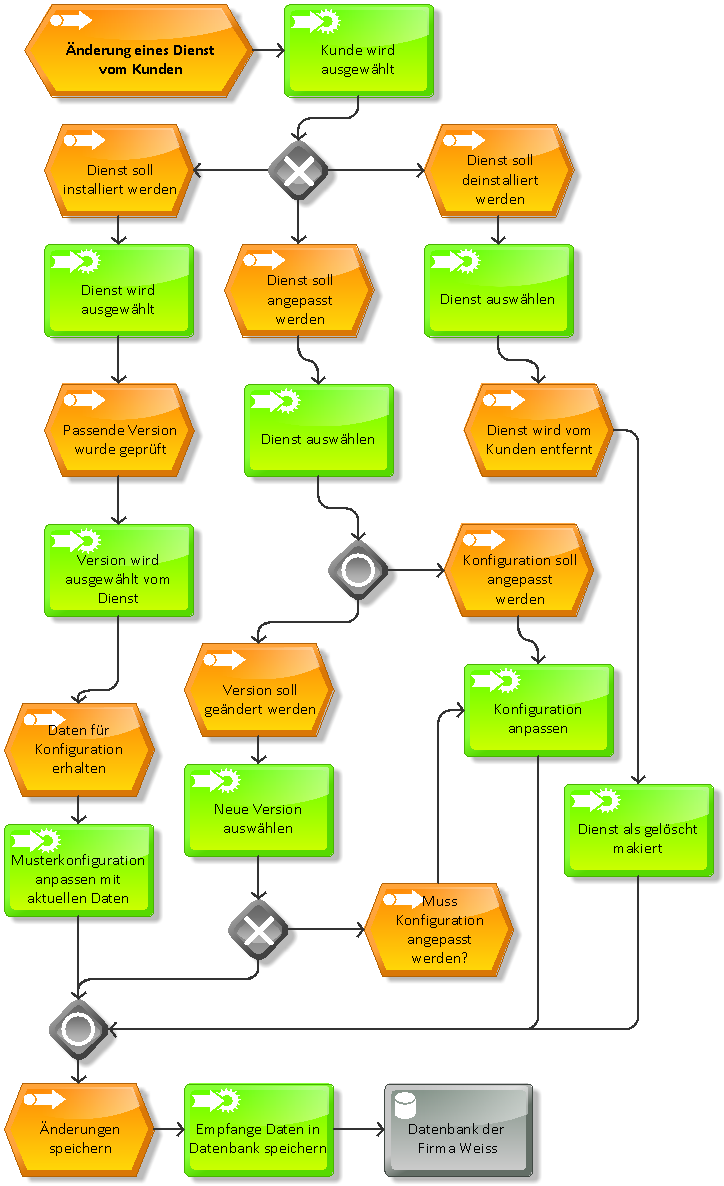
\includegraphics[scale=0.45]{content/attachments/GP_Service_Cltr.png}
\end{center}


\subsubsection{Dienstprüfung}
\label{app.useCase_check}

\begin{center}
    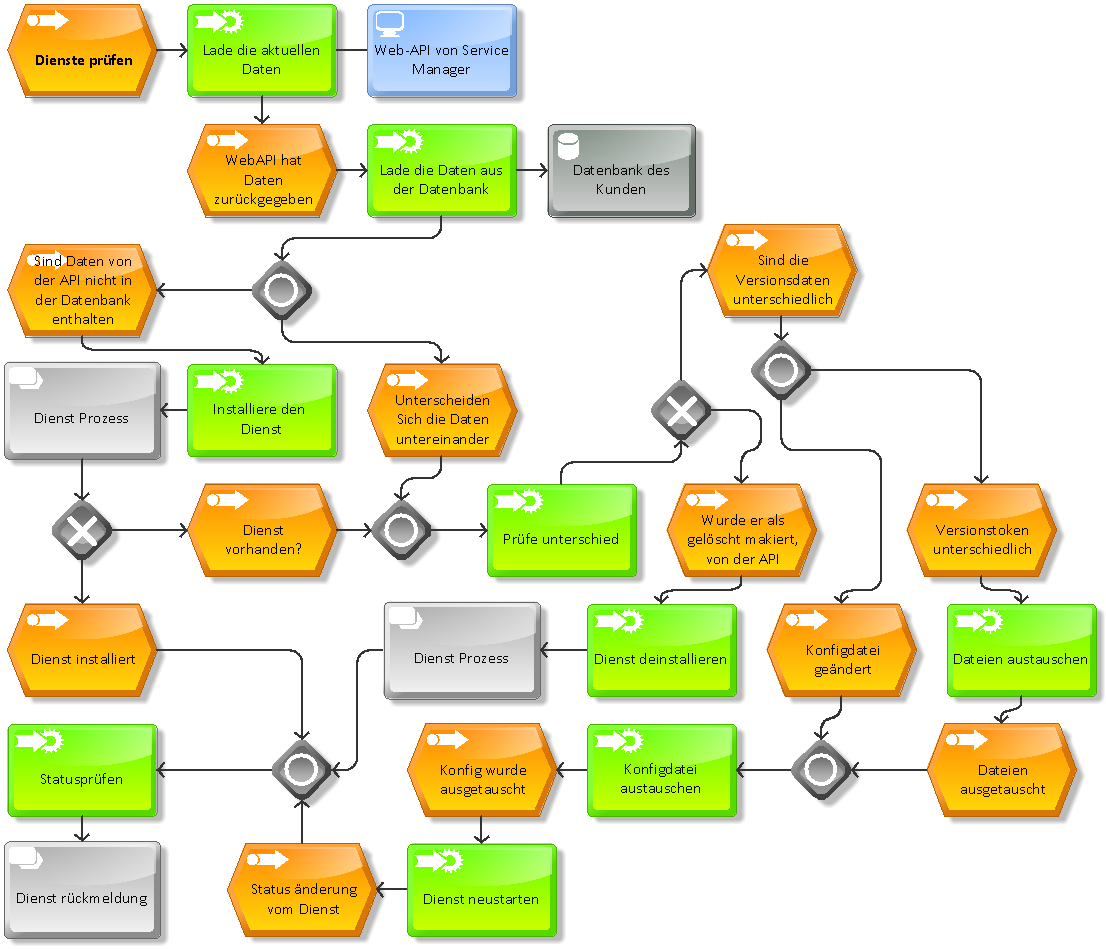
\includegraphics[scale=0.4]{content/attachments/GP_Service_Check.png}
\end{center}

\subsection{Oberfläche}
\label{app:view}

\subsubsection{Konzept}
\label{app:view_conc}

\begin{center}
    \begin{figure}[H]
        \centering
        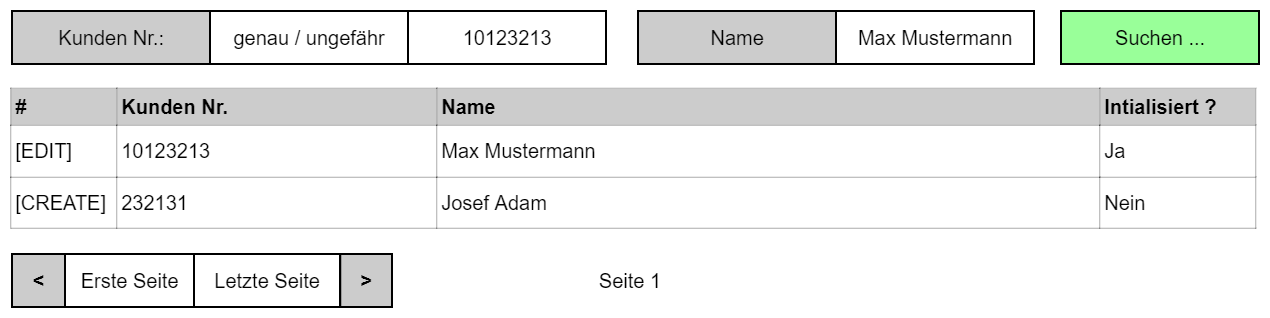
\includegraphics[scale=0.3]{content/attachments/k-cus-list.png}
        \caption{Kundenliste}
        \label{fig:k_cus_list}
    \end{figure}
    
    \begin{figure}[H]
        \centering
        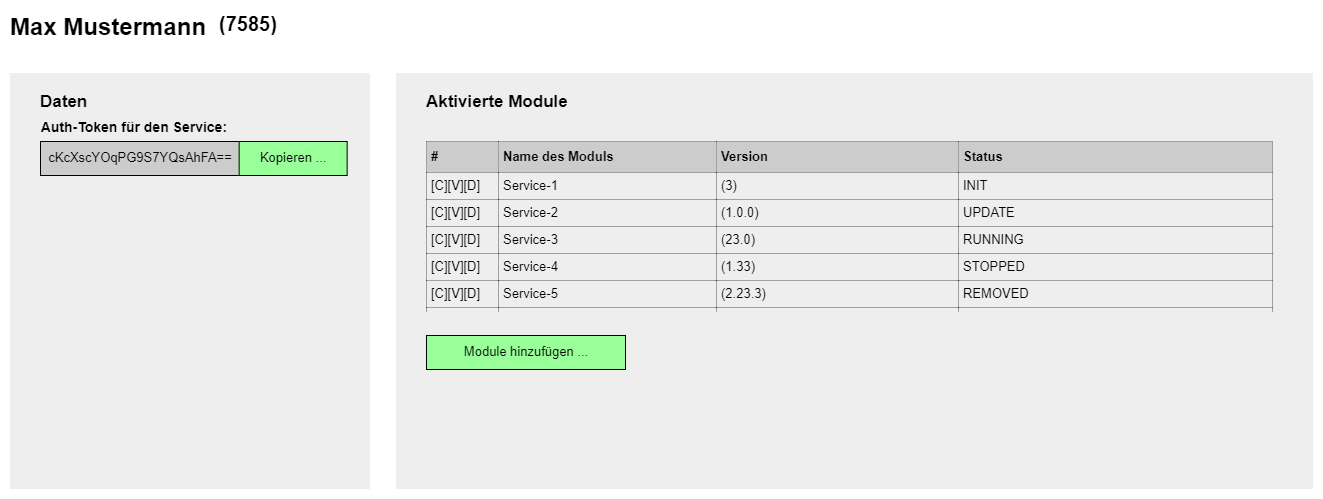
\includegraphics[scale=0.3]{content/attachments/k-cus-view.png}
        \caption{Kundenansicht}
        \label{fig:k_cus_view}
    \end{figure}
    
    \begin{figure}[H]
        \centering
        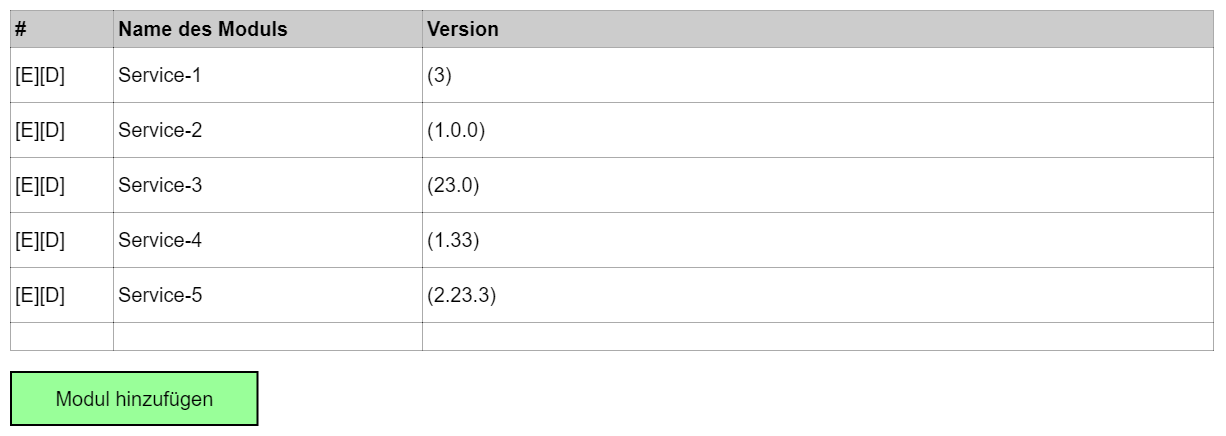
\includegraphics[scale=0.3]{content/attachments/k-ser-list.png}
        \caption{Dienstliste}
        \label{fig:k_ser_list}
    \end{figure}
    
    \begin{figure}[H]
        \centering
        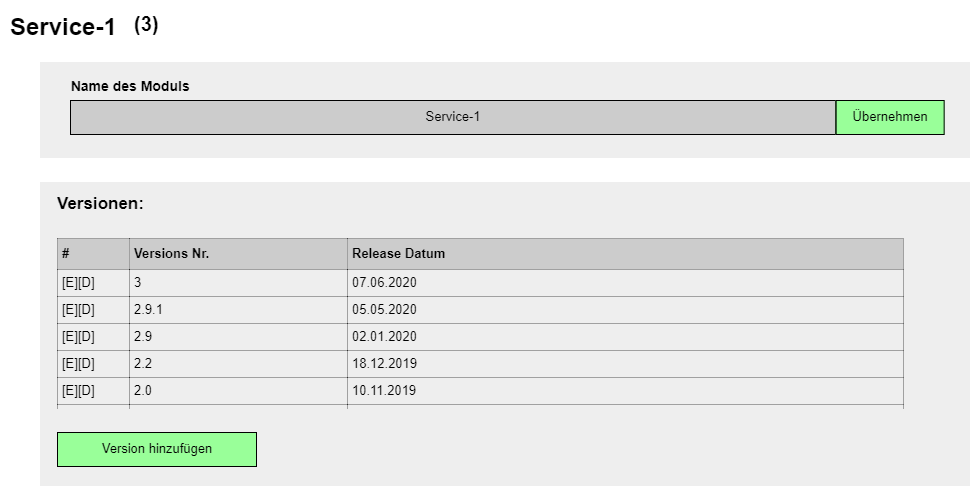
\includegraphics[scale=0.4]{content/attachments/k-ser-view.png}
        \caption{Dienstansicht}
        \label{fig:k_ser_view}
    \end{figure}
    
    \begin{figure}[H]
        \centering
        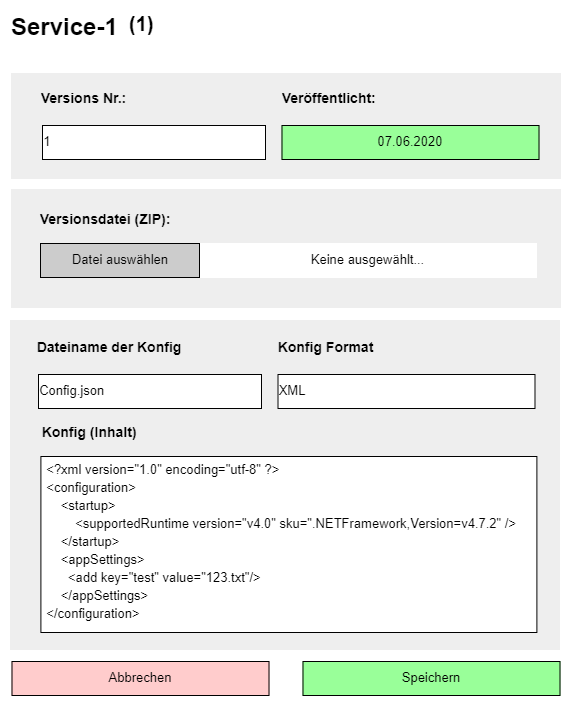
\includegraphics[scale=0.4]{content/attachments/k-ver-view.png}
        \caption{Versionseditor}
        \label{fig:k_ver_list}
    \end{figure}
\end{center}

\newpage

\subsubsection{Echtsystem}
\label{app:view_real}

\begin{center}
    \begin{figure}[H]
        \centering
        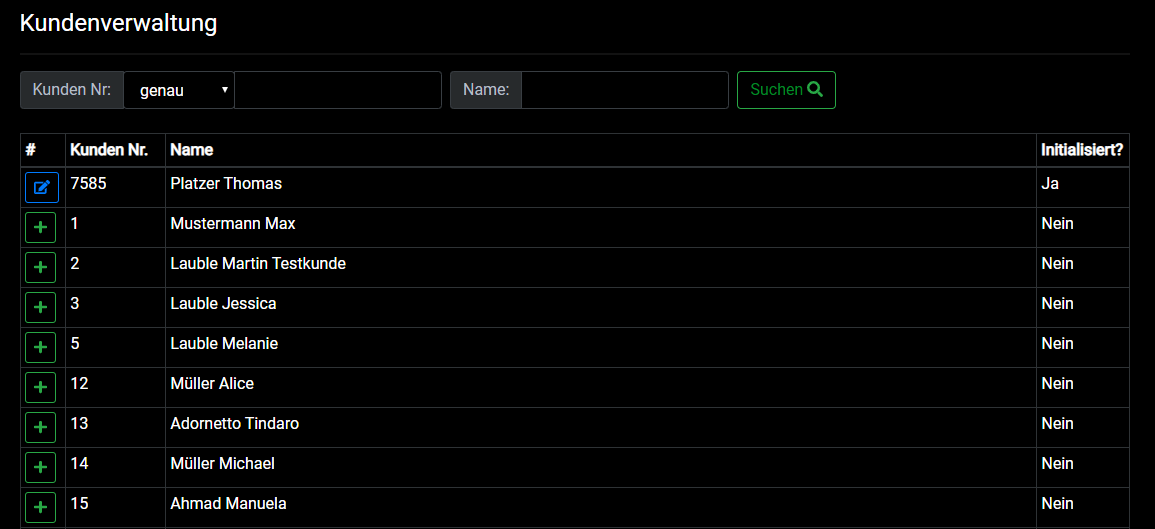
\includegraphics[scale=0.4]{content/attachments/s-cus-list.png}
        \caption{Kundenliste}
        \label{fig:s_cus_list}
    \end{figure}
    
    \begin{figure}[H]
        \centering
        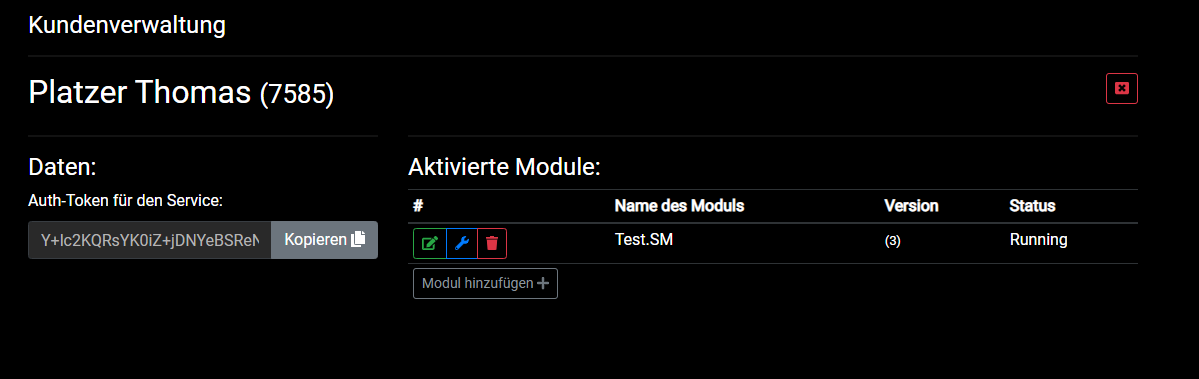
\includegraphics[scale=0.4]{content/attachments/s-cus-view.png}
        \caption{Kundenansicht}
        \label{fig:s_cus_view}
    \end{figure}
    
    \begin{figure}[H]
        \centering
        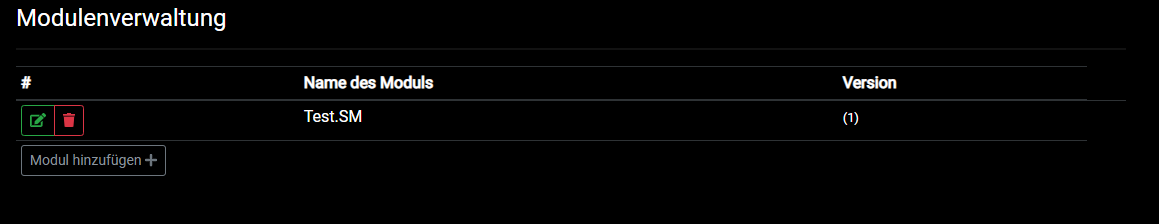
\includegraphics[scale=0.4]{content/attachments/s-ser-list.png}
        \caption{Dienstliste}
        \label{fig:s_ser_list}
    \end{figure}
    
    \begin{figure}[H]
        \centering
        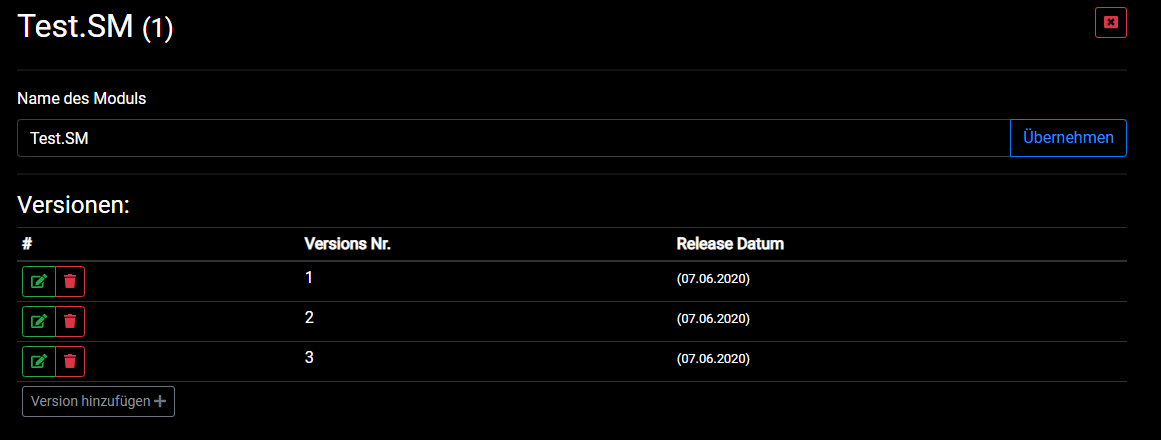
\includegraphics[scale=0.4]{content/attachments/s-ser-view.png}
        \caption{Dienstansicht}
        \label{fig:s_ser_view}
    \end{figure}
    
    \begin{figure}[H]
        \centering
        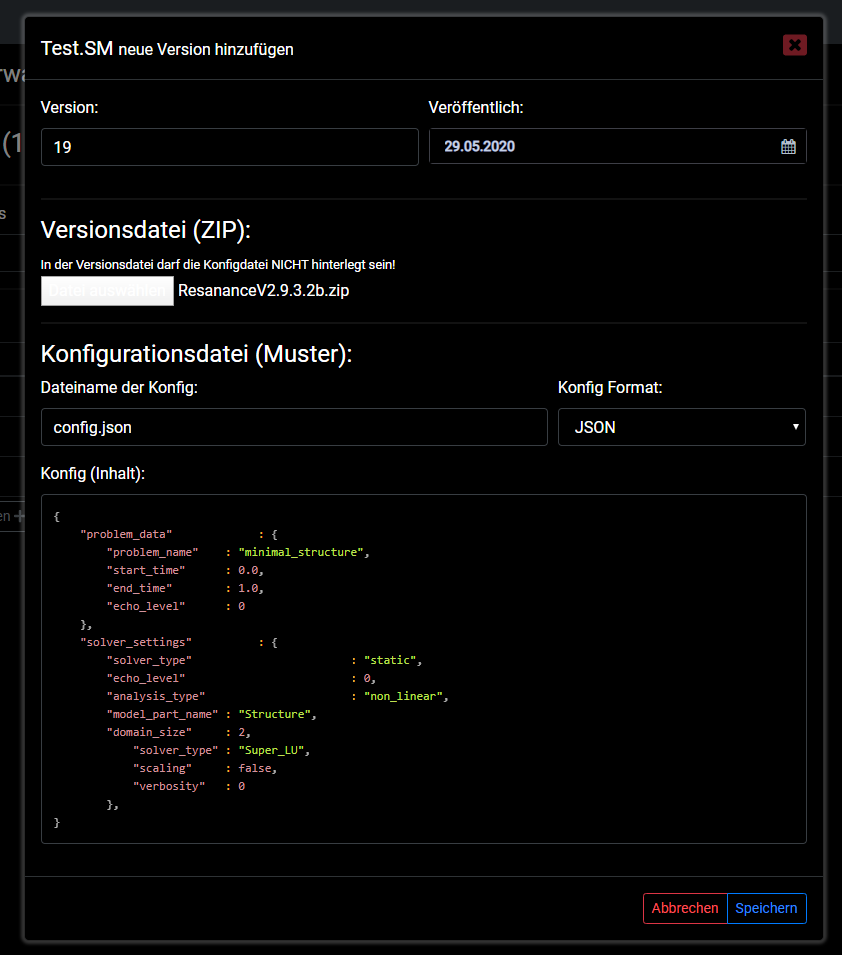
\includegraphics[scale=0.4]{content/attachments/s-ver-view.png}
        \caption{Versionseditor}
        \label{fig:s_ver_list}
    \end{figure}
\end{center}

\subsection{Klassendiagramme}
\label{app:class_concept}

\begin{center}
    \begin{figure}[H]
        \centering
        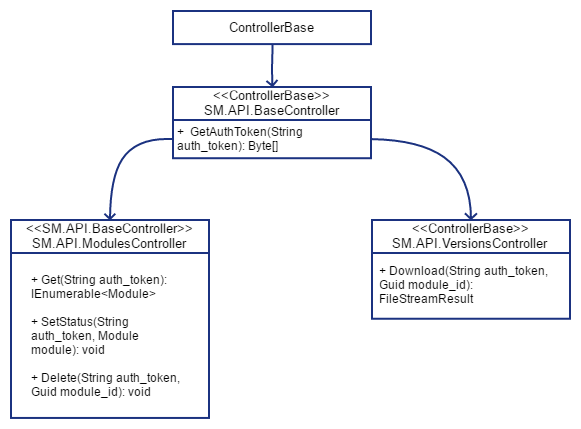
\includegraphics[scale=0.4]{content/attachments/c-api-cntrl.png}
        \caption{Controller-Klassen der API Anwendung}
        \label{fig:c-api-cntrl}
    \end{figure}
    
    \begin{figure}[H]
        \centering
        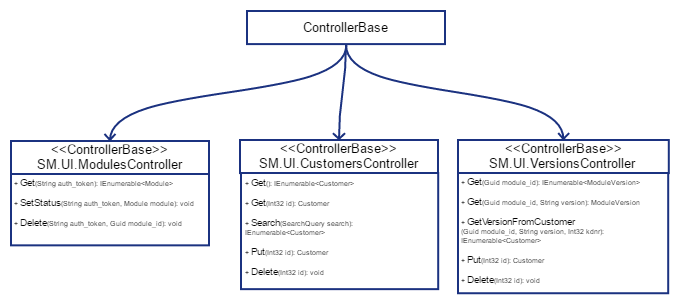
\includegraphics[scale=0.4]{content/attachments/c-ui-cntrl.png}
        \caption{Controller-Klassen der Oberflächen/UI Anwendung}
        \label{fig:s_cus_view}
    \end{figure}
\end{center}

\subsection{Tabellenmodell}
\label{app:database_table}

\begin{center}
    \begin{figure}[H]
        \centering
        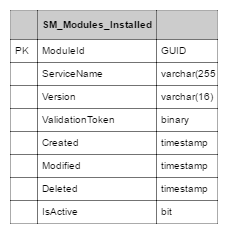
\includegraphics[scale=0.4]{content/attachments/d-table-cus.png}
        \caption{Tabelle die in der Kunden-Datenbank ist}
        \label{fig:d-table-cus}
    \end{figure}
    
    \begin{figure}[H]
        \centering
        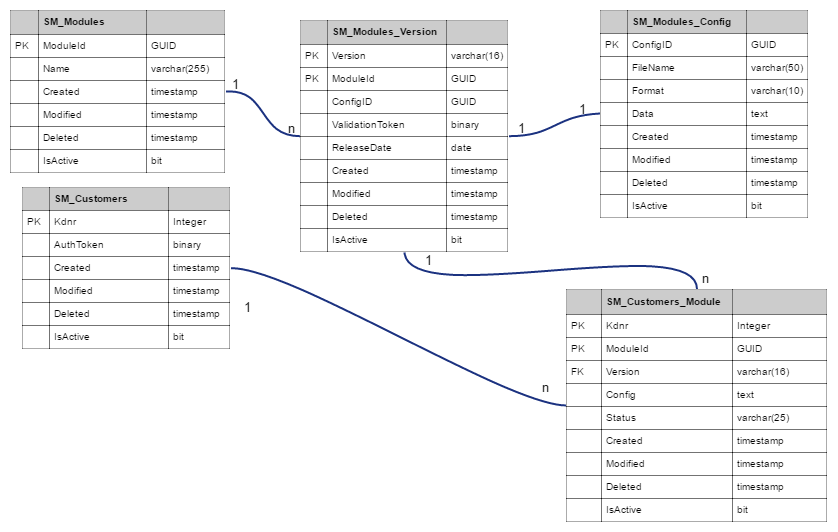
\includegraphics[scale=0.4]{content/attachments/d-table-wss.png}
        \caption{Tabellen in der Datenbank der Firma Weiss}
        \label{fig:d-table-wsss}
    \end{figure}
\end{center}

\subsection{Quellcode}
\label{app:sourceCode}

\begin{center}
 \lstinputlisting
    [caption={Quellcode zum importieren der Funktionen, um Dienste verwalten zu können}
       \label{lst:import-cs},
       captionpos=t,language=CS]
 {content/code/p-import.cs}
 
 \lstinputlisting
    [caption={Quellcode um Dienste installieren zu können (DLLs müssen importiert sein!)}
       \label{lst:install-cs},
       captionpos=t,language=CS]
 {content/code/p-install.cs}
 
 \lstinputlisting
    [caption={Quellcode zum entfernen der Dienste (DLLs müssen importiert sein!)}
       \label{lst:delete-cs},
       captionpos=t,language=CS]
 {content/code/p-delete.cs}
\end{center}


\end{document}